\documentclass{article}
\usepackage[utf8]{inputenc}

\title{TT3010 - Audio technology and room acoustics. \newline Exercise 4 - Loudspeakers in rooms.}

%\author{Jan Arne Bosnes}
\date{\today}

\usepackage{natbib}
\usepackage{graphicx}
\usepackage{multicol}
\usepackage{gensymb}
\usepackage{float}


\begin{document}

\maketitle

All tasks are retrieved from chapter 24 in  "Science of Sound". It is recommended that the student will try to do every task, but tasks marked \textit{Mandatory}, are to be handed in for approval (online). The deadline is specified in blackboard.

\section*{Tasks}
%\begin{multicols}{2}
\begin{itemize}
    \item [1.] At what frequency does the wavelength of sound equal the diameter in a 15-in. (38 cm) woofer? What about a 2-in. (5 cm) tweeter?
        
    \item[2.] \textit{Mandatory.} Assuming the outdoor sound system described in 24.12 (useful only for the comparison at the end) were to convert 2.5 kW of electrical power to acoustic power with an average efficiency of 20\% and to radiate it into a 90\degree angle ($Q$=4), determine the sound pressure level at 90 m. (First determine $L_W$ for the source.) Compare this to the design level at this distance.
        
    \item[3.] What are the upper and lower frequencies passed by an octave-band filter tuned to 500 Hz? (In other words, what frequencies are one-half octave above and below 500 Hz?)
    
    %\item[4.] \textit{Not relevant for this course} If we assume the record and playback heads are spaced 1 cm apart, what tape speed is required to give a delay time of 20 ms? Is this practical?
    
    
    \item[4.] If a microphone is 5 m in front of a loudspeaker, at what frequency might oscillation take place due to acoustic feedback? Could it also occur at harmonics of this frequency? Explain.
        
    \item[5.] It has been said that it would take 50 speakers 5 years to generate enough energy to boil a cup of tea. Can you confirm this statement? (\textit{Hint:} It takes about 1050 J to raise the temperature of a 0.25 liter cup of water 1\degree C; a joule is equal to watt-seconds(Ws), if needed don't hesitate to make your own assumptions)

    
    \item[6.] \textit{Mandatory.} A sound source having $Q$ = 2 and a sound power level $L_W = 80$ dB radiates into a room with total absorption $A$=500 m$^2$.
    
    \begin{itemize}
        \item [a.] Using figure \ref{fig:curve}, find the sound pressure level $L_p$ at distances of 5 m  and 15 m from the source.
        \item [b.] Make the same computations using Eq. (\ref{eq:spl}).
    \end{itemize}
    
  

\end{itemize}

%\end{multicols}

  \begin{equation}
        L_p = L_W + 10\log(\frac{Q}{4 \pi r^2} + \frac{4}{A})
        \label{eq:spl}
    \end{equation}

\begin{figure}[H]
    \centering
    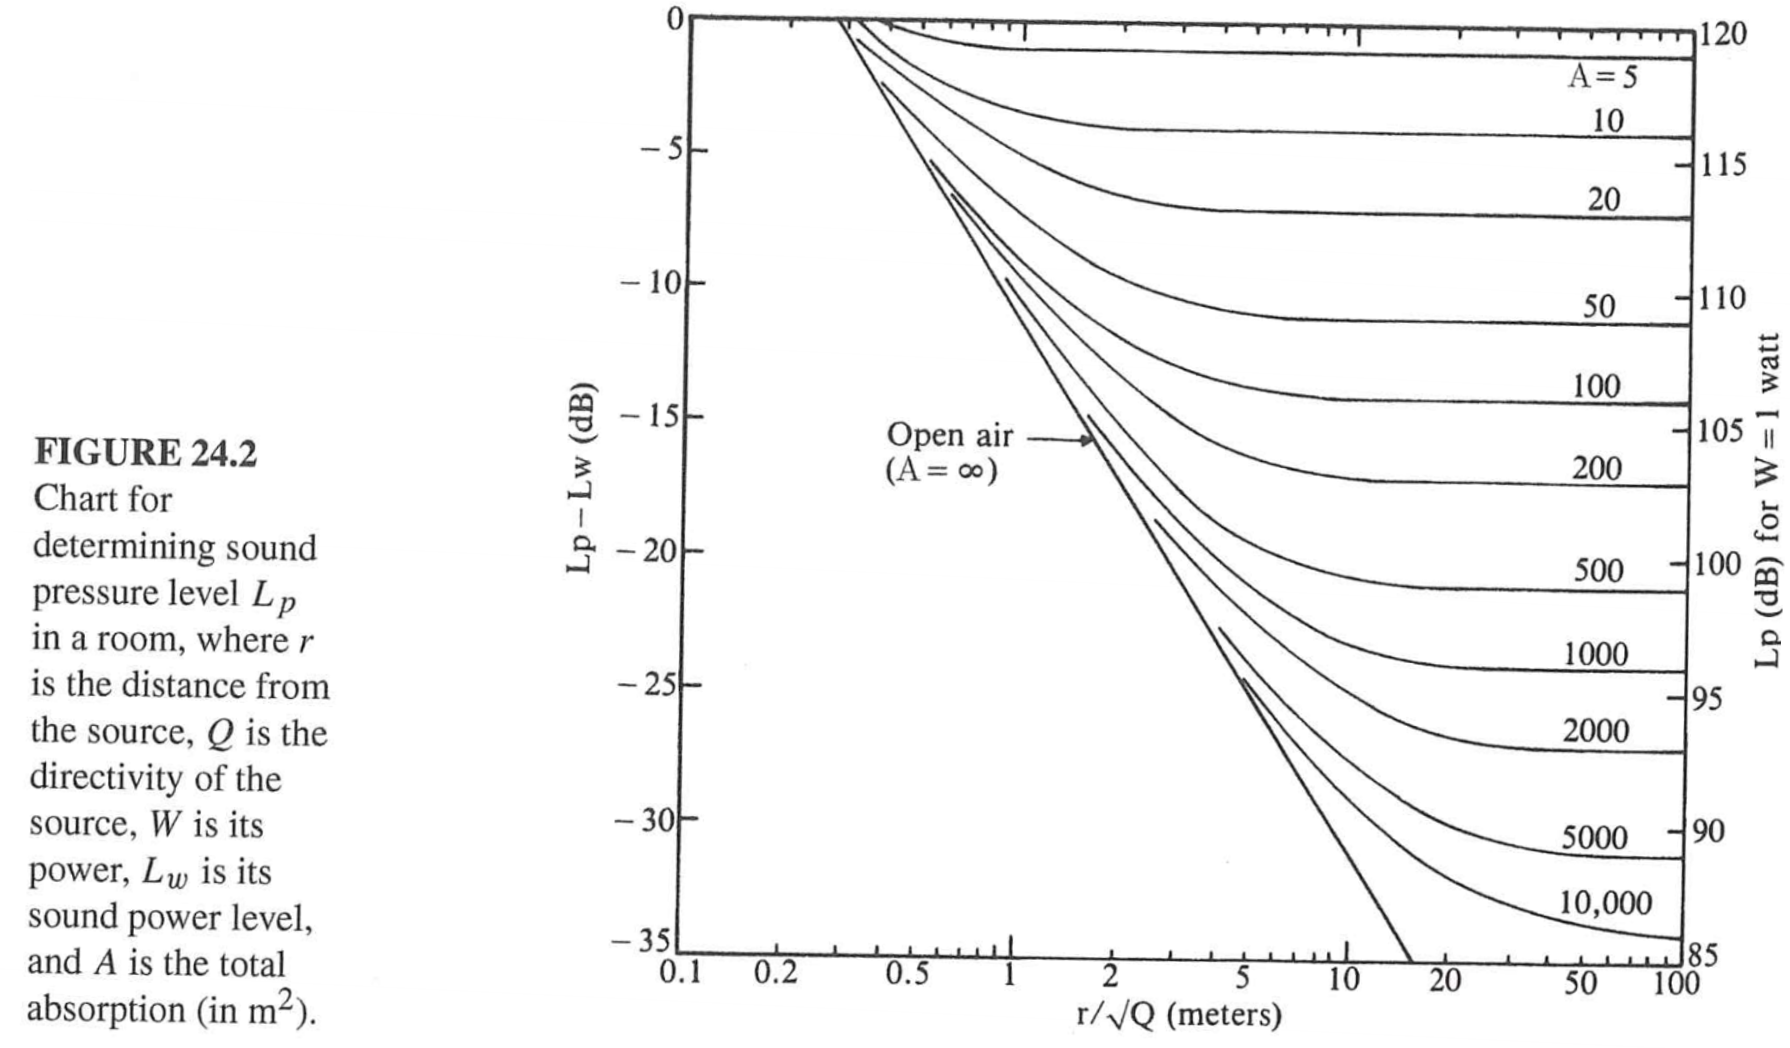
\includegraphics[scale=0.7]{figures/oving2_1.png}
    \caption{Illustration from "Science of Sound", chap 24.}
    \label{fig:curve}
\end{figure}

\end{document}